\documentclass[MS]{inithesis}
%\documentclass[economy,twoside,bind]{inithesis}
% Use the second for a single-spaced copy suitable for duplex printing
% and binding.

% Other useful options (there are more options documented in Chapter 2):
%  * draft -- don't actually include images, print a black bar on overful
%             hboxes
%  * MS    -- Format for a Master's Thesis.  No UMI abstract page, some 
%             textual changes to title page.  


% Useful packages for thesis writing:
\usepackage[greek,english]{babel}
\usepackage[utf8]{inputenc}
\usepackage{float}
\usepackage{amsmath, amssymb, amsfonts, amsthm}
\usepackage{graphicx}
\usepackage{listings}
\usepackage{xcolor}
\usepackage{csquotes}
% Define a custom style named 'customgo'
\lstdefinestyle{customgo}{
    language=Go,
    xleftmargin=\parindent,
    basicstyle=\ttfamily\footnotesize,
    backgroundcolor=\color{gray!10},  % Background color
    commentstyle=\color{teal},        % Comments in teal
    keywordstyle=\color{blue},        % Regular keywords in blue
    stringstyle=\color{red},          % Strings in red
    showstringspaces=false,
    showspaces=false,
    numbers=left,                     % Line numbers on the left
    numberstyle=\tiny\color{gray},    % Line numbers in tiny gray font
    numbersep=5pt,
    tabsize=4,
    breaklines=true,
    breakatwhitespace=true,
    frame=single,                     % Single frame around code
    morekeywords=[2]{trigger_event, current_task_id, next_task_id, task_attribute_value, task_id, task_type, task_attribute},  % Additional keywords for class 2
    morekeywords=[3]{double_value, list_value, waypoints_id_value, integer_value, string_value},  % Additional keywords for class 3
    morekeywords=[4]{...},  % Additional keywords for class 3
    keywordstyle=[2]{\itshape\color{orange}},  % Class 2 keywords in italic orange
    keywordstyle=[3]{\itshape\color{blue}},   % Class 3 keywords in italic purple
    keywordstyle=[4]{\itshape\color{green}}
}
\lstdefinestyle{c1}{
    language=Matlab,
    xleftmargin=\parindent,
    basicstyle=\ttfamily\footnotesize,
    backgroundcolor=\color{gray!10},  % Background color
    commentstyle=\color{teal},        % Comments in teal
    keywordstyle=\color{blue},        % Regular keywords in blue
    stringstyle=\color{red},          % Strings in red
    showstringspaces=false,
    showspaces=false,
    numbers=left,                     % Line numbers on the left
    numberstyle=\tiny\color{gray},    % Line numbers in tiny gray font
    numbersep=5pt,
    tabsize=4,
    breaklines=true,
    breakatwhitespace=true,
    frame=single,                     % Single frame around code
    morekeywords=[2]{trigger_event, current_task_id, next_task_id, task_attribute_value, task_id, task_type, task_attribute},  % Additional keywords for class 2
    morekeywords=[3]{double_value, list_value, waypoints_id_value, integer_value, string_value},  % Additional keywords for class 3
    morekeywords=[4]{...},  % Additional keywords for class 3
    keywordstyle=[2]{\itshape\color{orange}},  % Class 2 keywords in italic orange
    keywordstyle=[3]{\itshape\color{blue}},   % Class 3 keywords in italic purple
    keywordstyle=[4]{\itshape\color{green}}
}

\usepackage{xcolor}  % Optional, for coloring code
%\usepackage{natbib}
\usepackage{color}
\usepackage{bm}
%\usepackage{subfigure}
\usepackage{graphicx}
\usepackage{mathabx}
\usepackage{multirow}
\usepackage{setspace}
\usepackage{pdfpages}
\usepackage{tocloft}
\addtolength\cftfignumwidth{2.7em}%
\addtolength\cfttabnumwidth{2.7em}%
%\renewcommand{\cftpartnumwidth}{4em}
%\renewcommand{\cftchapaftersnumb}{\hspace{0em}}
%\renewcommand{\cftsecnumwidth}{1.5em}
%\renewcommand{\cftsecaftersnumb}{\hspace{0em}}
%\renewcommand{\cftsubsubsecindent}{8em}
%\renewcommand{\cftsubsecaftersnumb}{\hspace{0em}}

% \usepackage{cite}  % If you include this, hyperlink cites will
                     % break.  It's nice to use this package if your bibstyle
							% sorts entries by order-of-use, rather than
							% alphabetically (as plain does).
							
%Theorem, Lemma, etc. environments
\newtheorem{theorem}{Theorem}%[section]
\newtheorem{lemma}[theorem]{Lemma}
\newtheorem{proposition}[theorem]{Proposition}
\newtheorem{corollary}[theorem]{Corollary}
\newtheorem{result}[theorem]{Result}

% Personal commands and abbreviations.
%Define and personal commands here

%Graphics Path to find your pictures
\graphicspath{{./Pictures/}}



%-----------------------------------------------------------------------------%
% PREAMBLE 
%-----------------------------------------------------------------------------%
\author{Xiangliang Chen}% First Name, Middle Initial, Last Name
\title{Domain Specific Language for Drone Autonomy}
%\supervisor{Dr. Nicolas Christin}
%\advisor{Dr. Nicolas Christin}
\department{Information Networking Institute} 
\program{Information Networking}% MSISTM, MSIN or MIST-X
\departmenthead{Dr. Dena Haritos Tsamitis}
\dean{Dr. Pradeep Khosla}
\previousdegreelist{B.S.Applied and Computational Math Sciences: Discrete Mathematics and Algorithms, University of Washington}% Separate Multiple Entries with ' \\ '
\fulldate{March, 2024} % Month, Year
% Year the degree was/will be conferred
\degreeyear{2024}

% Copyright text.  If undefined, default is 'All rights reserved'
% (Example sets the text to a hyperlinked Creative Commons Licence)
\copyrighttext{All Rights Reserved}



%-----------------------------------------------------------------------------%
% HYPERREF: plain black hypertext references for ref's and cite's.
%-----------------------------------------------------------------------------%

\usepackage[pdftex, pdfusetitle, plainpages=false, bookmarks, bookmarksnumbered,
            colorlinks, linkcolor=black, citecolor=black,
            filecolor=black, urlcolor=black]{hyperref}

\begin{document}

% Fill in the blanks in cur_ThesisSig.doc with your information and save in 
% PDF format as signature.pdf 
% 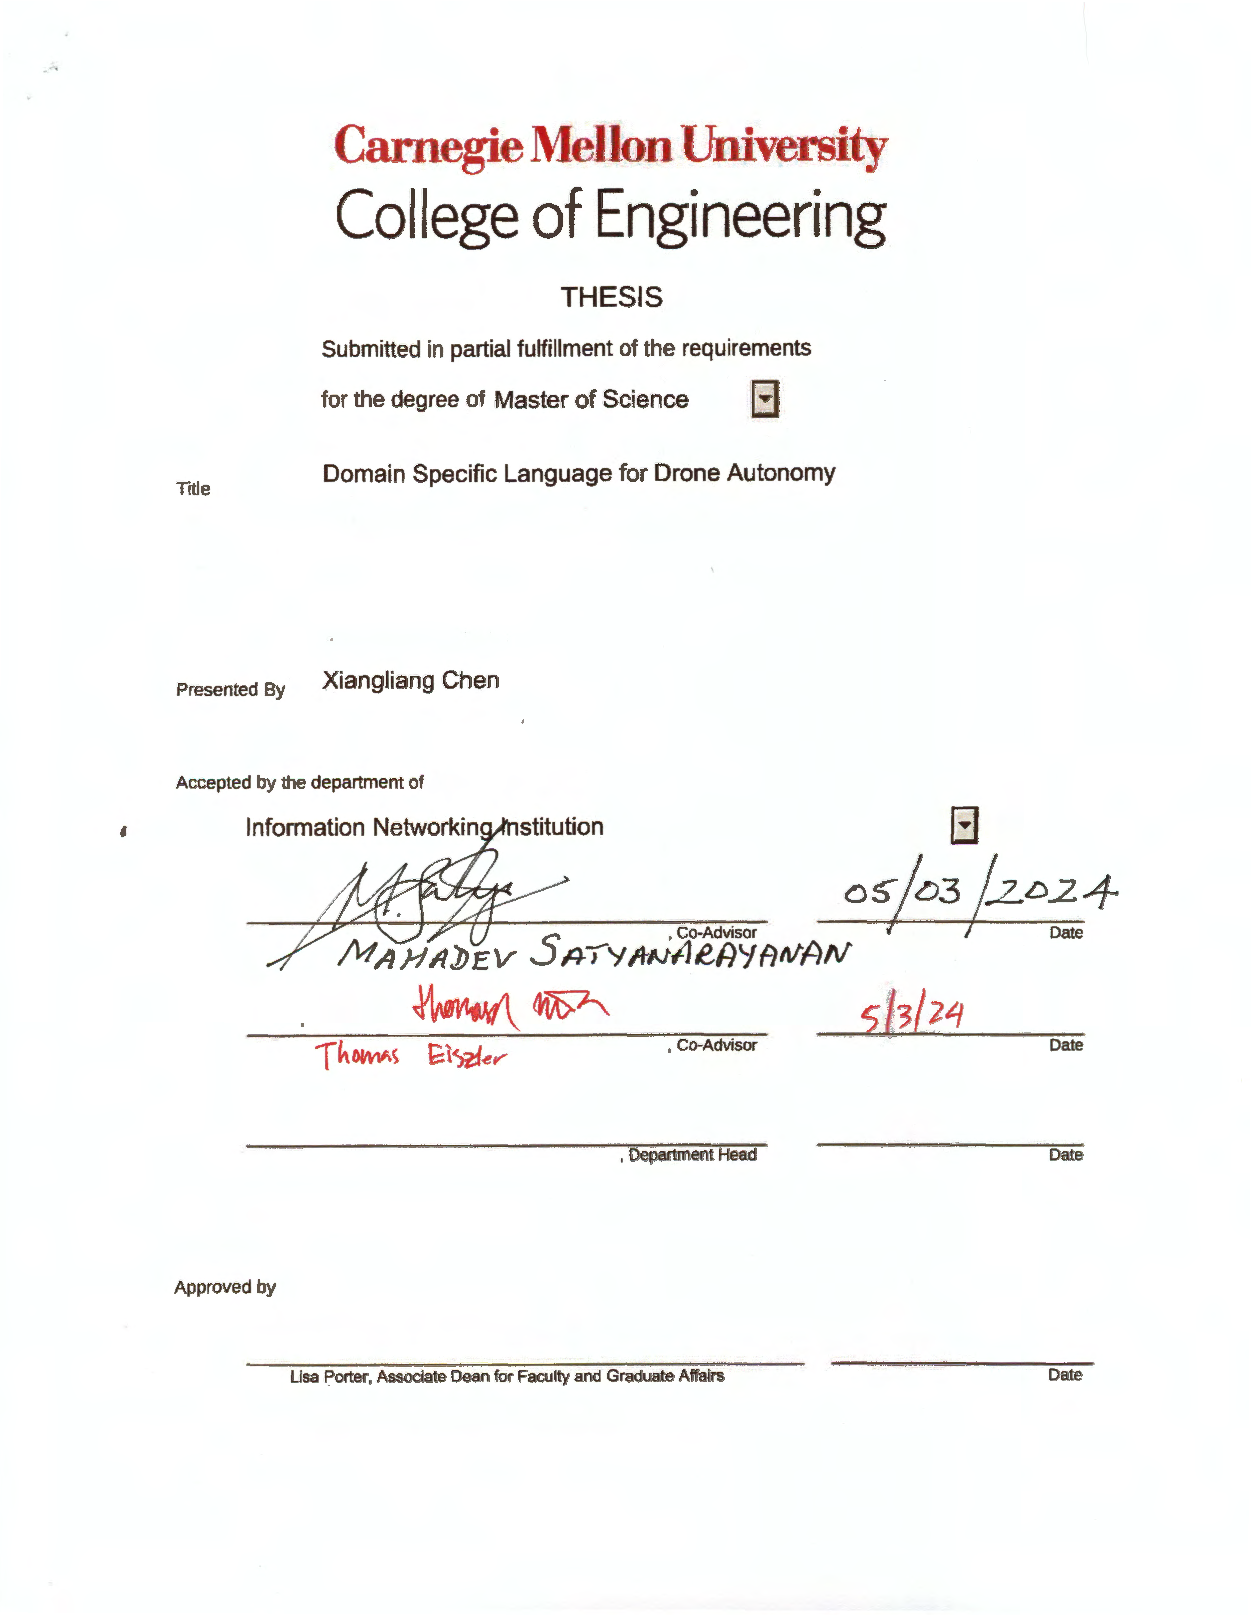
\includepdf[pages={1}]{signature.pdf}

%-----------------------------------------------------------------------------%
% TITLE PAGE -- provides UMI abstract title page & copyright if appropriate
%-----------------------------------------------------------------------------%
\maketitle

%-----------------------------------------------------------------------------%
% ACKNOWLEDGEMENTS -- included file should start with '\acknowledgements'
%-----------------------------------------------------------------------------%
\acknowledgements

\setcounter{page}{2}

I would like to thank Dr. Mahadev Satyanarayanan for his guidance as my primary advisor, and Thomas Eiszler Jr. and Mihir Bala for their support throughout my research. Thanks to Dr. Dena Haritos Tsamitis and the Information Networking Institute for allowing me to pursue a thesis-based degree.

I appreciate the SteelEagle group for implementing and testing my language in their pipeline. I'm grateful to my friends, especially Telsa Zhang, for their support during this project. Lastly, thank you to my family for their love and encouragement, even from a distance.

This material is based upon work supported by the U.S. Army Research Office and the U.S. Army Futures Command under Contract No. W519TC-23-C-0003, and by the National Science Foundation under grant number CNS-2106862. The content of the  information does not necessarily reflect the position or the policy of the government and no official endorsement should be inferred.
This work was done in the CMU Living Edge Lab, which is supported by Intel, Arm, Vodafone, Deutsche Telekom, CableLabs, Crown Castle, InterDigital, Seagate, Microsoft, the VMware University Research Fund, IAI, and the Conklin Kistler family fund. Any opinions, findings, conclusions or recommendations expressed in this document are those of the author and do not necessarily reflect the view of the above funding sources.}

%-----------------------------------------------------------------------------%
% ABSTRACT -- included file should start with '\abstract'.
%-----------------------------------------------------------------------------%
\abstract
This thesis introduces DroneDSL, a domain-specific language designed to enhance drone mission planning, especially for reconnaissance operations. The current state of drone mission planning has two main challenges. The first challenge stems from the complexity of integrating software and hardware functionalities, which complicates operations for pilots and limits the potential for code reusability among developers. To address this, DroneDSL offers an abstraction layer, simplifying interaction with drone systems and promoting developer efficiency through reusable code modules. The second challenge involves the need for dynamic mission execution capable of supporting complex logical operations such as looping and conditional execution, which surpass the capabilities of existing drone-specific languages designed for straightforward, linear mission plans. By incorporating a finite state machine, DroneDSL enables drones to adapt their missions dynamically in response to changing conditions, significantly enhancing the expressiveness and effectiveness of drone operations in reconnaissance and beyond.}

%-----------------------------------------------------------------------------%
% FRONTMATTER -- ToC is required, LoT and LoF are required if you have any
% tables or figures, respectively. List of Abbreviations and Symbols is 
% optional.
%-----------------------------------------------------------------------------%
% HYPERREF should be loaded last


% Correct usage of \phantomsection and \addcontentsline
\tableofcontents
\newpage

% \phantomsection
% \listoftables
% \addcontentsline{toc}{chapter}{List of Tables}
% \newpage

\phantomsection
\listoffigures
\addcontentsline{toc}{chapter}{List of Figures}
\newpage
%\abbreviations

% You can put here what you like, but here's an example
%Note the use of starred section commands here to produce proper division
%headers without bad '0.1' numbers or entries into the Table of Contents.
%Using the {\verb \begin{symbollist} } environment ensures that entries are
%properly spaced.

\section*{Symbols}

Put general notes about symbol usage in text here.  Notice this text is
double-spaced, as required.

\begin{symbollist}
	\item[$\mathbb{X}$] A blackboard bold $X$.  Neat.
	% Optional item argument makes the symbol/abbr
	\item[$\mathcal{X}$] A caligraphic $X$.  Neat.
	\item[$\mathfrak{X}$] A fraktur $X$.  Neat.
	\item[$\mathbf{X}$] A boldface $X$.
	\item[$\mathsf{X}$] A sans-serif $X$. Bad notation.
	\item[$\mathrm{X}$] A roman $X$.
\end{symbollist}

\section*{Abbreviations}

Long lines in the \texttt{symbollist} environment are single spaced, like in
the other front matter tables.

\begin{symbollist}
	\item[AR] Aqua Regia, also known as hydrocloric acid plus a splash of 
	nitric acid.
	\item[SHORT] Notice the change in alignment caused by the label width
	between this list and the one above.  Also notice that this multiline
	description is properly spaced. 
	\item[OMFGTXTMSG4ME] Abbreviations/Symbols in the item are limited to
	about a quarter of the textwidth, so don't pack too much in there.
	You'll bust the margins and it looks really bad.
\end{symbollist}
} % List of Abbreviations. Start file with '\abbreviations'

%==============================================================================
%-----------------------------------------------------------------------------%
%
% MAIN BODY OF PAPER
%
%
%-----------------------------------------------------------------------------%
\chapter{Introduction}
\label{sec:intro}

This thesis introduces DroneDSL, a domain-specific language designed to enhance the effectiveness and efficiency of drone mission planning, particularly in reconnaissance operations. Current methods in drone mission planning face significant challenges, including the complexity of integrating software and hardware functionalities. These complexities not only complicate operations for pilots but also limit the potential for code reusability among developers. To address these issues, DroneDSL provides an abstraction layer that simplifies the interaction with drone systems and supports developer efficiency through reusable code modules.

Furthermore, existing drone-specific languages are primarily designed for straightforward, linear mission plans and do not support complex logical operations such as looping and conditional execution. DroneDSL addresses this gap by incorporating a finite state machine that enables dynamic mission execution. This allows drones to adapt their operations dynamically in response to changing conditions, significantly enhancing the expressiveness and operational capabilities of drones in reconnaissance missions and beyond.

\section{Contributions of the Thesis}
The primary contributions of this thesis are:
\begin{itemize}
    \item The development of DroneDSL, which abstracts away complex drone control issues and provides a platform for reusing code, thereby increasing developer productivity.
    \item Enhancement of the drone mission planning process through a language that supports complex logical structures like loops and conditionals, allowing for dynamic and adaptive mission execution.
\end{itemize}

\section{Overview}
The structure of this thesis is organized as follows:
\begin{itemize}
    \item \textbf{Chapter 2: Background} - Discusses the relevant concepts of drone technology, including their types, components, and the basic principles of drone operation.
    \item \textbf{Chapter 3: Problem Statement} - Identifies the challenges in current drone mission planning and outlines the research goals.
    \item \textbf{Chapter 4: Literature Review} - Reviews existing work in the area of domain-specific languages for drones and other robotic applications.
    \item \textbf{Chapter 5: Computational Model} - Describes the computational models used, including finite state machines and task automata, which are central to DroneDSL.
    \item \textbf{Chapter 6: DroneDSL} - Provides a detailed explanation of DroneDSL, including its syntax and operational semantics.
    \item \textbf{Chapter 7: Implementation} - Discusses the implementation details of DroneDSL, covering aspects from preprocessing and compilation to runtime execution.
    \item \textbf{Chapter 8: Future Work} - Outlines future directions for extending DroneDSL and enhancing its capabilities.
    \item \textbf{Chapter 9: Conclusion} - Concludes the thesis work.
    \item \textbf{Bibliography} - Lists the references used throughout the thesis.
    \item \textbf{Appendix A} - Includes supplementary materials or detailed information that supports the thesis.
\end{itemize}
}
\chapter{Background}
\label{hello}

This chapter provides a brief overview of drones, discussing their definition, prevalent types, and operational methods, including how they are flown and how missions are planned.

\begin{itemize}
    \item \textbf{Drone Introduction:} Discusses the features, functionalities, and focuses particularly on quadcopters.
    \item \textbf{How to Fly a Drone:} Elucidates methods for flying drones, specifically focusing on autonomous flight.
    \item \textbf{Layers of Abstractions:} Summarizes the entire drone flying pipeline with three abstract layers: autopilot, off-board control, and mission planning.
\end{itemize}

\section{Introduction to Drones}
\subsection{Definition of Drones}
Drones, also known as Unmanned Aerial Vehicles (UAV), are robotic vehicles that operate without human occupants. They are capable of manual or autonomous control and function in diverse environments.
This subsection introduces several popular types of drones, all of which can be configured and managed using open-source software for drone development \cite{px4docs2023} \cite{ardupilot2023}:
\subsection{Types of Drones}
This subsection introduces several popular types of drones:
\begin{itemize}
    \item \textbf{Multicopters:} Noted for their vertical takeoffs and ability to hover, though they are generally slower and have shorter flight durations. They are favored for their ease of assembly and effectiveness as camera platforms.
    \item \textbf{Helicopters:} Offer similar advantages to multicopters but are mechanically more complex and efficient, making them more challenging to operate.
    \item \textbf{Planes (Fixed-wing):} Capable of longer and faster flights than multicopters, ideal for extensive surveys but require greater piloting skill, especially for slow flight and landing.
    \item \textbf{VTOL (Vertical Takeoff and Landing):} Combines the features of multicopters and fixed-wing planes for vertical takeoffs and increased flight coverage but are complex and costly.
\end{itemize}
In this thesis, we only focus on multicopters, specifically quadcopters.

\subsection{Drone Components and Off-Board Devices}
\begin{itemize}
    \item \textbf{Flight Controller (FC):} The central component that runs autopilot software, linking sensors and actuators to control the drone.
    \item \textbf{Autopilots:} The operational "brain" of drones, running sophisticated software on real-time operating systems to manage flights.
    \item \textbf{Sensors:} Essential for autonomous operation, these include gyroscopes, accelerometers, and GPS to measure various parameters like position and orientation.
    \item \textbf{ESCs \& Motors:} Drones typically utilize brushless motors with Electronic Speed Controllers (ESCs) to modulate power output.
    \item \textbf{Battery/Power:} Powered by Lithium-Polymer (LiPo) batteries, with systems to distribute energy efficiently to components.
    \item \textbf{Manual Control:} Operated via Radio Control systems or joysticks, integrated with software like QGroundControl\cite{qgroundcontrol2023} for direct manipulation.
    \item \textbf{Ground Control Stations (GCS):} Facilities that enable operators to monitor and direct drone activities and its payloads.
\end{itemize}

\section{How to Fly a Drone}

Flying a drone autonomously involves several stages, from mission planning to real-time operation and monitoring. This section focuses specifically on autonomous flights controlled via off-board systems.

\subsection{Mission Planning}
The process begins with the pilot planning the mission:
\begin{itemize}
    \item \textbf{Route Planning:} The pilot draws the flight route on a map, defining specific waypoints.
    \item \textbf{Task Specification:} Alongside route planning, specific tasks are assigned, such as object detection at certain locations, data collection, or tracking a target.
\end{itemize}

\subsection{Mission Upload and Initiation}
Once the mission is planned:
\begin{itemize}
    \item \textbf{Uploading the Mission:} The plan is uploaded from the GCS to the drone via a communication protocol. This includes all routes, tasks, and necessary parameters for flight.
    \item \textbf{Autopilot Engagement:} The drone's onboard autopilot system, which operates the flight stack software, receives signals from the Ground Control Station (GCS) and directs the hardware accordingly.
\end{itemize}

\subsection{Execution and Monitoring}
During the mission execution:
\begin{itemize}
    \item \textbf{Autonomous Flight:} The drone follows the predefined path autonomously, executing the specified tasks using its onboard systems.
    \item \textbf{Data Transmission:} The drone continuously sends back real-time data to the GCS, which may include video feed, sensor data, and status updates.
    \item \textbf{Pilot Monitoring:} The pilot monitors the drone’s operations via the GCS, ready to intervene manually if necessary, to adjust the mission parameters or take direct control in response to unforeseen situations.
\end{itemize}

\subsection{Landing the Drone}
Landing is a critical phase in drone operation, whether it is done manually or autonomously:
\begin{itemize}
    \item \textbf{Selecting a Landing Spot:} Ensure the landing area is clear of obstacles and suitable for the drone to land safely.
    \item \textbf{Autonomous Landing:} If the drone is set to land autonomously, monitor the descent to make sure it proceeds as planned.
    \item \textbf{Manual Landing:} In manual mode, the pilot must carefully control the descent and touchdown to avoid damage.
\end{itemize}

\section{Layers of Abstraction in Drone Operation}

The operation of a drone, especially in complex autonomous missions, involves multiple layers of abstraction that help segregate responsibilities and simplify control mechanisms.

\subsection{Autopilot Layer}
The lowest layer in the drone’s operational hierarchy:
\begin{itemize}
    \item \textbf{Function:} Direct control over the drone's actuators and sensors, managing basic flight operations such as stabilization, altitude control, and navigation.
    \item \textbf{Examples of Autopilot Software:} Popular open-source autopilots include PX4 \cite{px4docs2023}, ArduPilot \cite{ardupilot2023}, and iNav \cite{inavflight2023}, each providing a robust platform for various types of drones and missions.
\end{itemize}

\subsection{Off-Board Control Layer}
Serves as the intermediary layer:
\begin{itemize}
    \item \textbf{Role:} Facilitates communication between the drone and the GCS, transmitting commands and receiving telemetry data.
    \item \textbf{Popular Protocols:} MAVLink \cite{mavlink2023}, ROS (Robot Operating System) \cite{rosdocs2023}, UAVCAN \cite{uavcan2023}, and UranusLink\cite{UranusLink} are widely used for their reliability and support for a range of hardware and software systems.
\end{itemize}

\subsection{Mission Planning Layer}
The highest layer focuses on mission design and execution strategy:
\begin{itemize}
    \item \textbf{Mission Scripting:} Utilizes formats like KML (Keyhole Markup Language) \cite{kmltutorial2023} to script and layout missions, specifying waypoints, actions, and flight tasks.
    \item \textbf{Capabilities:} While KML is predominantly used for geographical data representation, it is adapted in GCSs like QGroundControl \cite{qgroundcontrol2023} to plan and execute complex drone operations.
\end{itemize}

\subsection{Conclusion}
Understanding these layers of abstraction helps clarify how drones operate autonomously and interact with control systems, highlighting the sophistication of modern drone technology and the continuous improvements needed in software and communication protocols to enhance operational efficiency and safety.
} % A regular chapter, starts with '\chapter{Title}'
\chapter{Problem Statement}
\label{sec:ProblemStatement}

This chapter delves into the specifics of current drone mission planning processes, particularly focusing on reconnaissance missions, and identifies the limitations of existing scripting methods like KML in addressing the dynamic requirements of such missions. This discussion sets the stage for proposing a domain-specific language tailored to overcome these challenges.

\section{Popular Drone Missions}
Drone missions encompass a range of activities, including surveillance, cargo transport, and infrastructure inspection. Reconnaissance missions, in particular, demand a high level of adaptability and self-awareness from drones to respond effectively to changing environmental conditions.

\section{Mission Planning and Challenges}
As outlined in Chapter 2, the predominant scripting language for drone missions is KML, a tag-based structure with nested elements designed primarily for geographical data representation. However, KML falls short in several areas crucial for effective drone mission planning:
\begin{itemize}
    \item \textbf{Dynamic Behavior:} KML lacks mechanisms to express dynamic behaviors and is not suited for conditional branching or looping, essential for complex mission scenarios.
    \item \textbf{Cognitive Load:} The language's nested structure can  obscure the understanding and management of missions.
\end{itemize}

\section{Research Goals}
While KML provides valuable engineering benefits such as encapsulation of implementation details, compilation checking, and script simplicity and reusability, it lacks the expressiveness needed to model the dynamic behaviors of drones effectively. This thesis proposes the design of a new domain-specific language (DSL) that retains the advantageous abstraction layer of KML while enhancing expressiveness to allow pilots to model drone behaviors accurately. The design goals for this new DSL include:
\begin{itemize}
    \item \textbf{Expressiveness:} Sufficient to capture dynamic behaviors crucial for complex drone operations.
    \item \textbf{Platform Agnosticism:} Usable across different drone platforms.
    \item \textbf{User-Friendly:} Easy to learn and use, even for those with limited programming experience.
\end{itemize}

This new DSL aims to bridge the gap between the technical limitations of KML and the operational needs of drone missions, providing a robust tool for mission planning in diverse and dynamically changing environments.
}
\chapter{Literature Review}
\label{sec:Literature Review}

\section{State of the Art}

This chapter synthesizes key contributions to domain-specific languages (DSLs) for robotic applications, highlighting significant advancements in DSL design for adaptability, mission planning, and operational autonomy.

\textbf{Lucas Alves et al.} introduces DRESS-ML, a domain-specific language designed to enhance the modeling of drone-based applications by incorporating self-adaptive behaviors and exceptional situations, moving beyond traditional models that only account for expected flight plans and limited environmental conditions. Leveraging the principles of Behavior-driven development (BDD) and Aspect-oriented Programming (AOP), DRESS-ML allows for detailed specification of system behaviors and adaptation strategies to ensure resilience and continuous operation in diverse and unpredictable environments.  \cite{Alves2022DRESSML}.

\textbf{Davide Di Ruscio et al.} introduces a family of domain-specific languages designed to specify missions for multi-robot systems, focusing on creating models that are technology-independent, analyzable, executable, and extensible to new application areas. These languages aim to make robotic systems more accessible to non-technical operators by bringing the language closer to the problem domain, thus facilitating the democratization of robotics\cite{Ruscio}.

\textbf{Adrian Rutle et al.} presented CommonLang, a DSL for universal robot programming across varied hardware. Utilizing model-driven engineering, it converts high-level directives into robot-specific code, boosting programming efficiency and cross-platform interoperability \cite{Rutle}.

\textbf{André C. Santos et al.} introduced a DSL for adaptive mobile robot navigation, segregating adaptation logic from core application code to improve modularity and system maintainability. The language's flexibility was validated through smartphone-assisted navigation tests \cite{santos}.

\textbf{Flavia Cavalcanti et al.} presented "Flail: A Domain Specific Language for Drone Path Generation" proposed a novel approach for defining drone flight paths using an HTC Vive, enabling intuitive 3D trajectory design. This DSL simplifies flight control and was demonstrated through drone simulations and flight tests \cite{Cavalcanti}.

\textbf{Chao Cao et al.} introduced an aerial planning behavior tree, a structured approach to drone behavior management responding to environmental and internal states. This method supports autonomous real-time decision-making, optimizing mission execution and safety \cite{Cao}.
}
\chapter{Computational Model}
\label{sec:ComputationalModel}

This chapter explores the finite state machine computational model, illustrating the system's behavior and introducing a tailored version for drone mission planning known as Task Automata.

\section{Computational Model - Finite State Machine}
We briefly discuss the concept of finite state machines (FSM) and their application in modeling drone behaviors.

\subsection{State}
\begin{itemize}
    \item Indicates the agent's current activity and status.
    \item The agent executes relevant commands in its present state, managing operations from initiation to completion.
\end{itemize}

\subsection{Transition Function}
\begin{itemize}
    \item Manages the agent's state transitions in response to specific events.
    \item These events enable the agent to dynamically adjust its mission activities.
\end{itemize}

\subsection{Trigger Event}
\begin{itemize}
    \item Clearly defined within an FSM's design, each state change is associated with a particular event.
    \item Events can vary widely, from simple signals to complex conditional triggers.
\end{itemize}

The suitability of FSMs for drone missions is evident as they facilitate state transitions (or tasks) based on environmental cues or timed events detected by the drone, effectively managing the mission's workflow.

\section{Computational Model - Task Automata}
We delve into \textbf{Task Automata}, a state machine approach specifically designed for drone missions, breaking down the mission execution process and discussing each component in detail.



\subsection{State} In each mission, the drone agent begins at the \textbf{Start State}, transitions through various \textbf{Task States} via transition functions, and eventually terminates at the \textbf{Terminate State}.
\begin{itemize}
    \item \textbf{Start State:} This is where all missions start. It is a blank state that does not do anything but transitions.
    
    \item \textbf{Task State:}  This state defines an individual task to execute for the drone agent. When reached, it will execute all the specified task commands.
    \begin{itemize}

        \item \textbf{Detect Task:} This task instructs the drone to locate objects along a designated path using specific parameters. Completion occurs once the drone has navigated all specified waypoints.
        \item \textbf{Track Task:} This task directs the drone to continuously follow a specific object class, utilizing a selected model. The task is considered complete if the drone loses track of the target for a duration of 10 seconds.
        \item \textbf{Avoidance Task:} This task involves guiding the drone from one location to another while it avoids obstacles along a pre-set route. The task is completed when the drone reaches all the designated waypoints.

    \end{itemize}
    
    \item \textbf{Terminate State:} This is where all missions end. The drone agent will return to home in this state.
\end{itemize}



\subsection{Transition Function}
This section outlines the types of transition functions in Task Automata that direct state changes during drone operations.

\textbf{Transition Type:}
\begin{itemize}
    \item \textbf{Explicit Transition:} This transition is defined by the user.
    \begin{itemize}
        \item \textbf{Start Transition:} Transitions the drone unconditionally from the start state to a task state. There is only one start transition in Task Automata.
        \item \textbf{Task Transition:} Transitions the drone from one task state to another, triggered by a specified event.
    \end{itemize}

    \item \textbf{Implicit Transition:} If a task transition does not specify a subsequent task state to execute upon completion, the agent will implicitly transition to the terminate state after executing all commands within the current task state and without any further task transitions being triggered. If specified, the transition is considered invalid.
\end{itemize}

\subsection{Trigger Event}
A trigger event specifies under what circumstances the \textbf{Task Transition} will be triggered.

\textbf{Events in Drone Operation:}
\begin{itemize}
    \item \textbf{Timeout:} This event triggers after a specified duration of time has passed.
    \item \textbf{Detection:} This event triggers when a specified class of object is detected.
    \item \textbf{Done:} This event triggers when the task has reached its conclusion.
\end{itemize}


\section{Task Automata Evaluation}
This section evaluates the computational capabilities of Task Automata within the framework of drone mission planning.

\subsection{Computational Limitations and Strengths}
Task Automata, as a specialized form of finite state machine, is tailored for handling drone-specific tasks and scenarios. While it demonstrates significant strengths in managing state transitions based on environmental cues and mission-specific events, it inherently lacks the broader computational capabilities of more general models like Turing Machines. Task Automata does not support general-purpose programming features such as complex mathematical computations, general-type conditional branching, or concurrency. Furthermore, it does not include capabilities similar to malloc() or new() found in more expansive programming languages, nor is it designed to simulate the infinite tape of a Turing Machine. These limitations highlight that while Task Automata is effective within its domain, it is not Turing complete.

\subsection{Contextual Computational Completeness}
Considering the specific needs of drone mission planning, the design of Task Automata focuses on simplicity, efficiency, and effectiveness in a highly specialized context. Within the realm of drone operations, Task Automata may not need to simulate the infinite tape of a Turing Machine, as the scope and requirements of missions are usually well-defined and constrained. The primary goal is not expressiveness but operational efficiency and reliability.


\subsection{Implications for DroneDSL}
The specialized nature of Task Automata makes it a suitable model for DroneDSL, providing enough functionality to efficiently manage drone missions without the overhead of unnecessary complexity. This simplification results in better compile-time error checking and a more intuitive understanding for users who are experts in the domain rather than in programming. Thus, while DroneDSL and Task Automata sacrifice universal computational power, they gain in terms of accessibility and practical utility for specific applications.

\section{Conclusion}
Task Automata serves as an effective computational model for DroneDSL, balancing the needs of specialized drone mission planning with the simplicity required for practical application. Although not Turing complete, its design reflects a deliberate trade-off that prioritizes domain-specific efficacy over general computational flexibility.
}
\chapter{DroneDSL}
\label{sec:dronedsl}


\textbf{DroneDSL} is a domain-specific language carefully designed to streamline the programming of drone mission lifecycles. It assists users in defining drone behavior adaptively, abstracting complex underlying implementation details to produce executable code compatible with various drone platforms. In DroneDSL, each flight mission is structured as a task-based automaton (similar to a finite state machine), which orchestrates the drone's adaptation behaviors through a series of defined states and responsive events.

\section{File Structure}
The DroneDSL script is divided into two main sections, each serving a distinct purpose in setting up the mission.

\subsection{Overview} 
\begin{itemize}
    \item In the task section, the keyword \textbf{Task} is followed by braces, within which users define the task instances that determine the state in the task automata.
    \item In the mission section, the keyword \textbf{Mission} followed by braces allows users to define the transition functions from one task to another, creating transitions within the task automata.
\end{itemize}

\begin{lstlisting}[style=customgo]
Task {
    // Definition of task states
}

Mission {
    // Specification of transition functions
}
\end{lstlisting}




\section{Task Section }
This section is dedicated to defining the various task states that a drone can execute during its mission. Each task state details specific actions and settings.

\subsection{Task Definition}
Typically, we begin with the keyword \textbf{Detect}, \textbf{Track}, or \textbf{Avoid} followed by a \textit{\textbf{Task ID}} and braces. Within these braces, users must specify the task attributes related to the \textit{\textbf{Task Type}}. The necessary task attributes for each \textbf{\textit{Task Type}} are introduced in ~\ref{sec:task_type}.

\begin{lstlisting}[style=customgo]
Task{
    task_type task_id { // Definition of the task state
        task_attribute: task_attribute_value,  //  Attribute
        // Any attributes
        task_attribute: task_attribute_value,  
        task_attribute: task_attribute_value 
    }
     ... // Additional task state definitions
}
\end{lstlisting}


\subsection {Task type}
\label{sec:task_type}
Indicates the type of operation the drone will perform. Supported operations include: 
\begin{itemize}
    \item \textbf{Detect Task}\\
    Instruct drone to detect objects along the specified path using the specified pitch, rotation, sampling rate, and detection model\\
    \textbf{Required attributes:} \textit{Waypoints}, \textit{Gimbal Pitch}, \textit{Drone} \textit{Rotation}, \textit{Sample} \textit{Rate}, \textit{Hover} \textit{Delay}, \textit{Model}
    \begin{lstlisting}[style=customgo] 
    Detect task_id { // Definition of the task state
        waypoints: task_attribute_value,  //  waypoints
        gimbal_pitch: task_attribute_value,  // gimbal pitch
        drone_rotation: task_attribute_value,  // rotation
        sample_rate: task_attribute_value,  // sample rate  
        hover_delay: task_attribute_value, // hover delay
        model: task_attribute_value // model
    }
    \end{lstlisting}  
    
    \item \textbf{Track Task} \\
    Track specified class using a paritcular model for inferencing \\
    \textbf{Required attributes:} \textit{Gimbal Pitch, Model, Class}
    \begin{lstlisting}[style=customgo] 
    Track task_id { // Definition of the task state
        gimbal_pitch: task_attribute_value,  // gimbal pitch
        model: task_attribute_value, // model
        class: task_attribute_value // class
    }
    \end{lstlisting}  

    \item \textbf{Avoidance Task} \\
    Fly along the specified path while avoiding obstacles\\
    \textbf{Required attributes:} \textit{Waypoints, Model, Speed, Altitude}
    \begin{lstlisting}[style=customgo] 
    Avoid task_id { // Definition of the task state
        speed: task_attribute_value,  // speed
        model: task_attribute_value, // model
        altitude: task_attribute_value, // altitude
        waypoints: task_attribute_value // waypoints
    }
    \end{lstlisting}  
\end{itemize}

    
\subsection{Task ID} A unique alphanumeric identifier assigned to each task state. It supports Greek and Latin letters, underscores, digits, apostrophes, and hyphens. An identifier must start with a letter or underscore. Here are is the example where we name an avoidance task as \enquote{avoid\_task\_1}:
    \begin{lstlisting}[style=customgo]
    Avoid avoid_task_1 { // Definition of the task state
        speed: task_attribute_value,  // speed
        model: task_attribute_value, // model
        altitude: task_attribute_value, // altitude
        waypoints: task_attribute_value // waypoints
    }
    \end{lstlisting}


\subsection{Task attribute}Specifies the category of the task attribute. Available categories include:
    \begin{itemize}
        \item \textbf{Waypoints} \\
        The set of waypoints that drone agent need to reach in the mission flight route.
        \textbf{Type:} \textit{List},  \textit{Waypoint ID} 
        \begin{lstlisting}[style=customgo]
        // waypoints expressed as a list
        way_points: list_value

        // waypoints expressed as a waypoints ID
        way_points: waypoints_id_value
        \end{lstlisting}
        \item \textbf{Gimbal Pitch} \\
        The angle of a drone's camera gimbal along the vertical axis, allowing the camera to tilt up and down. Value must be greater or equal to -90.0 and lesser or equal to 90.0. \\
        \textbf{Type:} \textit{Double}
        \begin{lstlisting}[style=customgo]
        gimbal_pitch: double_value
        \end{lstlisting}
        \item \textbf{Drone Rotation} \\
        The heading offset to rotate the drone to at each vertex (in degrees) Value must be greater or equal to 0.0 and lesser or equal to 360.0. \\
        \textbf{Type:} \textit{Double}
        \begin{lstlisting}[style=customgo]
        drone_rotation: double_value
        \end{lstlisting} 
        \item \textbf{Speed} \\
        Speed to execute at. \\
        \textbf{Type:} \textit{Double}
        \begin{lstlisting}[style=customgo]
        speed: double_value
        \end{lstlisting}
        \item \textbf{Altitude} \\
        The altitude (above sea level) to fly at. \\
        \textbf{Type:} \textit{Double}
        \begin{lstlisting}[style=customgo]
        altitude: double_value
        \end{lstlisting}
        \item \textbf{Longitude}\\
        The longitude to fly at.\\
        \textbf{Type:} \textit{Double}
        \begin{lstlisting}[style=customgo]
        longitude: double_value
        \end{lstlisting}
        \item \textbf{Latitude} \\
        The latitude to fly at.\\
        \textbf{Type:} \textit{Double}
        \begin{lstlisting}[style=customgo]
        latitude: double_value
        \end{lstlisting}
        \item \textbf{Sample Rate} \\
        The number of frames to evaluate per second. Value must be greater or equal to 1 and lesser or equal to 30. \\
        \textbf{Type:} \textit{Integer}
        \begin{lstlisting}[style=customgo]
        sample_rate: integer_value
        \end{lstlisting}
        \item \textbf{Hover Delay} \\
        The number of seconds to hover at each waypoint before moving to the next. Value must be greater or equal to 0 and lesser or equal to 10. \\
        \textbf{Type:} \textit{Integer}
        \begin{lstlisting}[style=customgo]
        hover_delay: integer_value
        \end{lstlisting}
        \item \textbf{Model} \\
         Name of the Deep Neural Network (DNN) model used to evaluate frames. This name corresponds to a pretrained model that is invoked in the backend during runtime.\\
        \textbf{Type:} \textit{String}
        \begin{lstlisting}[style=customgo]
        model: string_value
        \end{lstlisting}
        \item \textbf{Class} \\
        Name of the class to track, relevant only in the context of the above model.\\
        \textbf{Type:} \textit{String}
        \begin{lstlisting}[style=customgo]
        class: string_value
        \end{lstlisting}

        
    \end{itemize}


\subsection{Primitive Type}
This subsection details the specific values associated with each task attribute, categorizing them by their data types:
\begin{itemize}
    \item \textbf{String}\\
    This type is used to represent textual data. For instance, it specifies the names of classes, models, and waypoint areas in a KML file.
    \item \textbf{Integer}\\
    Used for whole numbers. In this domain-specific language, integers specify values such as the sample rate and hover delay.
    \item \textbf {Double}\\
    A double precision floating-point number that is precise up to six decimal places. Commonly used to define geographical coordinates such as longitude, latitude, and altitude, as well as parameters like gimbal pitch, drone rotation, and speed.
    \item \textbf{Tuple}\\
    A collection of multiple values of the same type, bundled together. Typically, tuples are used to specify the coordinates of a waypoint as shown below
    \begin{lstlisting}[style=customgo]
    (double_value, double_value , double_value)  //Double is used to represent the value of longitude, latitude, and altitude.
    \end{lstlisting}
    
    \item \textbf{List}\\
    Utilized for specifying a sequence of waypoints. Each entry in the list is a tuple representing a waypoint. The format is as follows.
    \begin{lstlisting}[style=customgo]
    [(double_value, double_value, double_value), // Start of list
     ..., // Additional waypoints can be added here
     (double_value, double_value, double_value)] // End of list
    \end{lstlisting}
    
    \item \textbf{Waypoints ID}\\
    A unique identifier used to specify waypoints more conveniently without listing individual coordinates. This type helps users specify a named area of waypoints predefined in a KML file:
    \begin{lstlisting}[style=customgo]
    <string_value> // String is used to represent the name of waypoints area specified in KML
    \end{lstlisting}
\end{itemize}
    

\section{Mission}
This section outlines the transition functions between task states, which dictate the mission's flow based on specific events and conditions. There are two primary types of transitions: Start transitions and Task transitions. A Start transition moves the drone agent from the start state to the first task state. A Task transition moves the drone agent from one task state to another. If the drone agent completes the current task state without triggering any events, it will implicitly transition to the terminate state.

\subsection{Transition Definition}
\begin{itemize}
    \item \textbf{Start Transition} \\
    Start transition begins with the keyword \textbf{Start} followed by a task ID. User can only specify one start transition within the mission.
    \begin{lstlisting}[style=customgo]
    Mission{
        // Start transition
        Start task_id
    }
    \end{lstlisting}
    \item \textbf{Task Transition}\\
    Task transitions start with the keyword \textbf{Transition}, followed by parentheses containing the trigger event for the transition. Outside the parentheses, specify the current task ID from which the transition originates, followed by '\texttt{->}' and the next task ID to which the transition leads.
    \begin{lstlisting}[style=customgo]
    Mission{
        // Task transition
        // current task ID -> next task ID
        Transition (trigger_event) task_id -> task_id
        //... additional Task Transitions can be added here
    }
    \end{lstlisting}
\end{itemize}


\subsection{Trigger Event}
The trigger event is an argument in the transition function, defining the conditions under which a transition will be triggered. 

\begin{itemize}
    \item \textbf{Timeout}\\
    This event is triggered after a specified duration of time has passed.\\
    \textbf{Argument:} Integer value that specifies the seconds of the time need to be passed.
    \begin{lstlisting}[style=customgo] 
    timeout (integer_value) // integer argument
    \end{lstlisting}  
    
    \item \textbf{Object Detection}\\
    This event is triggered when a specified class of object is detected. Users can only specify this event to be triggered from the detect task state.\\
    \textbf{Argument:} String value that specifies the class name that needs to be detected.
    \begin{lstlisting}[style=customgo] 
    object_detection (string_value) // String argument
    \end{lstlisting}  

    \item \textbf{Done}\\
    This event is triggered when the task has reached its conclusion. Once the done event specified on the task state, it will override the implicit transition to the terminate state. Users can only specify this event to be triggered once for each task state.\\
    \textbf{Argument:} No Argument, the event will trigger when the task considered to be finished.
    \begin{lstlisting}[style=customgo] 
    done // No argument
    \end{lstlisting}  
\end{itemize}

% \section{Illustrative Examples of Task States}

% Detailed examples of task state definitions using DroneDSL:

% \begin{lstlisting}[style=customgo]
% Detect task1 {
%     way_points: <Triangle>,
%     gimbal_pitch: -45.0,
%     drone_rotation: 0.0,
%     sample_rate: 2,
%     hover_delay: 0,
%     model: coco
% }

% Detect task2 {
%     way_points: [(-79.9503492, 40.4155806, 25.0), (-79.9491717, 40.4155826, 25.0)],
%     gimbal_pitch: -45.0,
%     drone_rotation: 0.0,
%     sample_rate: 2,
%     hover_delay: 5,
%     model: none
% }
% \end{lstlisting}}
\chapter{Implementation}
\label{sec:implementation}

\section{Introduction}
This section has outlined the three essential modules that constitute the DroneDSL, covering the complete pipeline of the project. These modules are:
\begin{itemize}
    \item \textbf{Preprocessing}: Prepares the initial data and configurations needed for the subsequent stages.
    \item \textbf{Compilation}: Translates the DroneDSL script into an executable format, creating an Abstract Syntax Tree and subsequently generating a task automata structure.
    \item \textbf{Runtime}: Manages the execution of tasks during drone operations, overseeing the mission control and task transitions based on real-time condition.
\end{itemize}
\section{Preprocessing}
\subsection{Overview}
During this phase, the system processes a KML file to extract waypoints necessary for takeoff and flight tasks. These waypoints are bound to variable names designated by the user. In addition, users are required to compose their own DSL scripts to generate the configurations needed for their specific flight missions.
\begin{figure}[H] % The 'h' here is a placement specifier (here)
    \centering % This centers the figure
    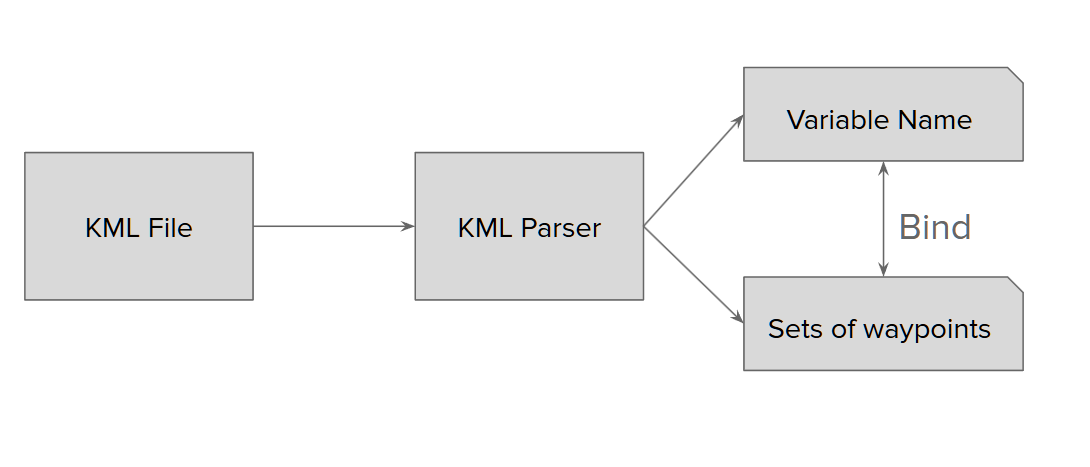
\includegraphics[width=0.8\textwidth]{Pictures/pre_flow.PNG}
    \caption{Workflow Diagram for Preprocess Module.}
    \label{fig:workflow_diagram}
\end{figure}

\subsection{Workflow}
\begin{itemize}
    \item Initially, users must generate the flight route using a mapping service or a ground control station.~\ref{fig:flight_route} is an example where Google My Maps is used to delineate a flight route for a mission.
    
    \begin{figure}[H] % The 'h' here is a placement specifier (here)
        \centering % This centers the figure
        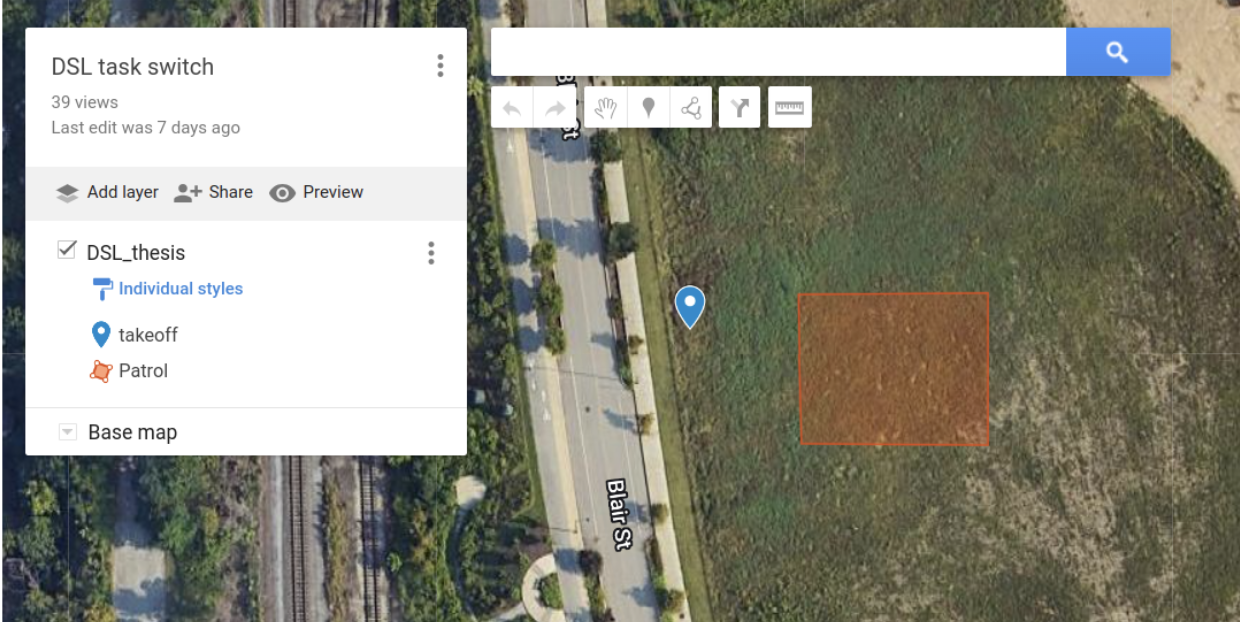
\includegraphics[width=0.8\textwidth]{Pictures/pre_qgc.PNG}
        \caption{Example of a flight route designed using Google My Maps.}
        \label{fig:flight_route}
    \end{figure}
    
    \item After the flight route is drawn, it is converted into a KML file. KML is retained in our pipeline due to its efficiency in expressing geographical information. It is used solely to represent waypoint information.~\ref{fig:kml_script} is a segment of the KML script that corresponds to the flight route illustrated in~\ref{fig:flight_route}.
    \begin{figure}[H] % The 'h' here is a placement specifier (here)
        \centering % This centers the figure
        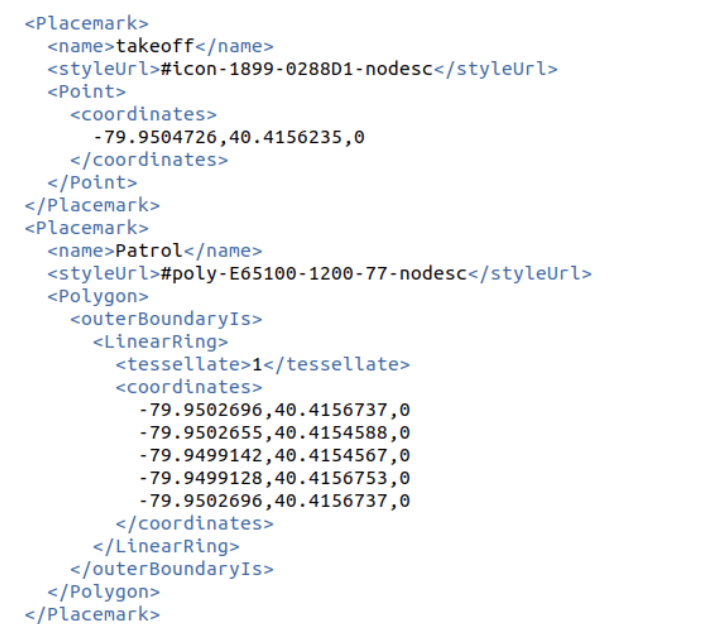
\includegraphics[width=0.8\textwidth]{Pictures/pre_kml.PNG}
        \caption{Snippet of the KML script for the depicted flight route.}
        \label{fig:kml_script}
    \end{figure}
    \item Once the KML file is obtained, the DroneDSL utilizes a KML parser to extract the waypoints and the names of the areas associated with these waypoints. These details are then bound together, allowing users to reference a set of waypoints using a single Waypoints ID. This approach significantly reduces the cognitive effort required to input each waypoint manually. ~\ref{fig:workflow_diagram} illustrates the workflow following the acquisition of the KML file.
\end{itemize}


\section{Compilation}
\subsection{Overview}
The DroneDSL script is interpreted into an Abstract Syntax Tree (AST). This AST is subsequently transformed into a Task Automata data structure in memory, which is then converted into a format suitable for integration with drone software development kits (SDKs).~\ref{fig:cli_flow} depicts the entire workflow of the compilation process.
\begin{figure}[H] % The 'h' here is a placement specifier (here)
    \centering % This centers the figure
    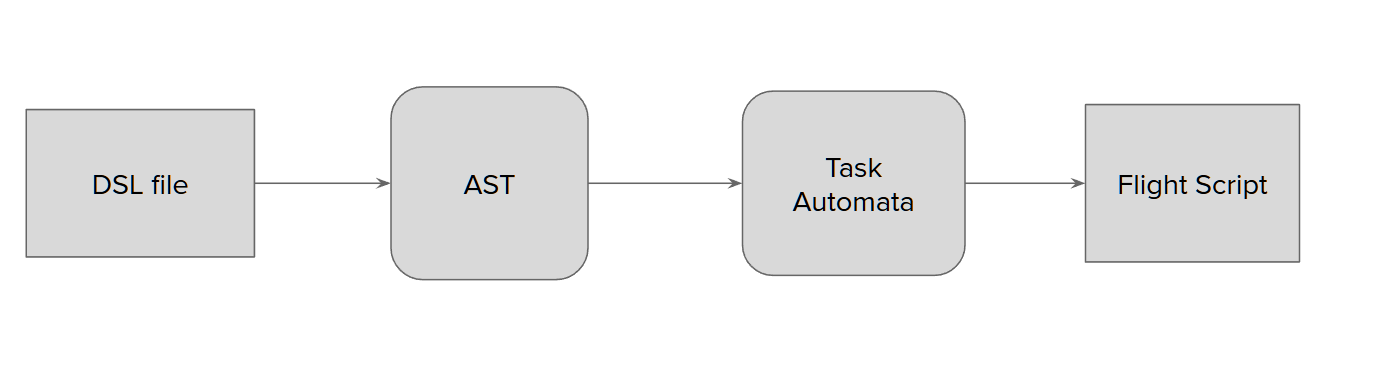
\includegraphics[width=0.8\textwidth]{Pictures/cli_flow.PNG}
    \caption{Workflow Diagram for Compilation Module.}
    \label{fig:cli_flow}
\end{figure}
\subsection{Compiler Details}
\subsubsection{Lexical Analysis}
The lexical analyzer processes the DroneDSL input and generates tokens based on the following specifications:
\begin{itemize}
    \item \textbf{Number}: Identifies integers and floating-point numbers. It matches an optional negative sign followed by one or more digits, possibly including a decimal point followed by more digits.
    \item \textbf{Identifier}: Recognizes identifiers comprising Greek (\textgreek{α}-\textgreek{ω}) and Latin (a-zA-Z) letters, underscores, digits, apostrophes, and hyphens, starting with a letter or underscore.
    \item \textbf{EOL}: Represents end-of-line characters.
    \item \textbf{White Space}: Defines whitespace characters, including spaces and tabs.
    \item \textbf{Keywords and Symbols}: Captures DSL keywords such as "Task," "Detect," "Track," "Mission," "Transition," "Start" and symbols like \texttt{\{ \} ( ) [ ] , : -> < >}.
    \item \textbf{Bad Character}: This rule captures any character input that does not match any of the specified patterns.
\end{itemize}

\begin{lstlisting}[style=c1]
    EOL=\R
    WHITE_SPACE=\s+
    NUMBER=-?[0-9]+(\.[0-9]+)?
    IDENTIFIER=
        [(alpha)-(omega)a-zA-Z_][(alpha)-(omega)a-zA-Z0-9_'-]*
    
    %%
    <YYINITIAL> {
      {WHITE_SPACE}       { return WHITE_SPACE; }
      {NUMBER}            { return NUMBER; }
      Task                { return TASK_KW; }
      Detect              { return TASK_DETECT_KW; }
      Track               { return TASK_TRACK_KW; }
      Avoid               { return TASK_AVOID_KW; }
      Mission             { return MISSION_KW; }
      Transition          { return TRANSITION_KW; }
      Start               { return MISSION_START_KW; }
      {IDENTIFIER}        { return ID; }
      "{"                 { return LBRACE; }
      "}"                 { return RBRACE; }
      "("                 { return LPAREN; }
      ")"                 { return RPAREN; }
      "["                 { return LSQUA; }
      "]"                 { return RSQUA; }
      ","                 { return COMMA; }
      ":"                 { return COLON; }
      "->"                { return ARROW; }
      "<"                 { return LANGL; }
      ">"                 { return RANGL; }
    }
    
    [^] { return BAD_CHARACTER; }
\end{lstlisting}

\subsubsection{Parsing}
DroneDSL uses context free grammar to define constructs for files, tasks, and missions, with components like task name, attribute, and mission transition. Each major component is structured as follows:
\begin{itemize}
    \item File Structure
    \begin{itemize}
        \item File: A file consists of a task followed by a mission.
    \end{itemize}
    \begin{lstlisting}[style=customgo]
    // file structure
    file ::= task mission
    \end{lstlisting}
    
    \item Task Definition
    \begin{itemize}
        \item \textbf{Task}: Defined by a keyword (TASK\_KW) followed by a series of task declarations (task\_decl) enclosed in braces.
        \item \textbf{Task Declaration}: A declaration can be for detecting, tracking, or avoiding (TASK\_DETECT\_KW, TASK\_TRACK\_KW, TASK\_AVOID\_KW), followed by a Task Name and a Task Body.
        \item \textbf{Task Body}: Consists of attributes separated by commas and enclosed in braces.
        \item \textbf{Attribute}: A sequence of attributes where each attribute is identified by an ID followed by a colon and an attribute expression.
        \item \textbf{Attribute Expression}: The expression for an attribute, which could be a number, a name, a list of waypoints, a waypoints variable, etc.
        \item \textbf{Task Name and Name}: Both are defined as IDs.
    \end{itemize}
    \begin{lstlisting}[style=customgo]
    // defining the task
    task ::= TASK_KW <<braced task_decl*>>
    task_decl ::= (TASK_DETECT_KW | TASK_TRACK_KW) task_name task_body
    task_body ::= <<braced <<commaSep attributes>>>>
    private attributes ::= attribute*
    attribute ::=  ID <<coloned attribute_expr>>
    attribute_expr ::= NUMBER | name | <<square_bracked <<commaSep <<paren tuple>> >> >> | <<angle_bracked name>> | <<paren tuple>>
    tuple ::= NUMBER COMMA NUMBER COMMA NUMBER
    task_name ::= name
    name ::= ID
    \end{lstlisting}    
    \item Mission Definition
    \begin{itemize}
        \item \textbf{Mission}: Defined by a keyword (MISSION\_KW) followed by content enclosed in braces.
        \item \textbf{Mission Content}: Consists of a mission\_start\_decl followed by zero or more mission\_transitions.
        \item \textbf{Start Transition}: Starts with a keyword (MISSION\_START\_KW) followed by a task\_name.
        \item \textbf{Task Transition}: Defined by a TRANSITION\_KW, a condition in parentheses, a task\_name, an arrow (ARROW), and another task\_name.
        \item \textbf{Transition Argument}: A condition which is an ID possibly followed by a number or another ID in parentheses.
    \end{itemize}
    \begin{lstlisting}[style=customgo]
    // defining the mission
    mission ::= MISSION_KW <<braced mission_content>>
    mission_content ::= mission_start_decl mission_transition*
    mission_start_decl ::= MISSION_START_KW task_name
    mission_transition ::= TRANSITION_KW <<paren cond>> task_name ARROW task_name
    cond ::= ID <<paren (NUMBER | ID) >>?
    \end{lstlisting}
    \item Meta Rules \\
    These rules define how lists and groups are structured:
    \begin{itemize}
        \item \textbf{Parentheses}: Content enclosed in parentheses.
        \item \textbf{Angle Brackets}: Content enclosed in angle brackets.
        \item \textbf{Square Brackets}: Content enclosed in square brackets.
        \item \textbf{Colon}: A colon followed by some content.
        \item \textbf{Comma Separation}: A comma-separated list of items.
        \item \textbf{Braces}: Content enclosed in braces.
    \end{itemize}
    \begin{lstlisting}[style=customgo]
    // meta rules
    meta paren ::= LPAREN <<param>> RPAREN
    meta angle_bracked ::= LANGL <<param>> RANGL
    meta square_bracked ::= LSQUA <<param>> RSQUA
    private meta coloned ::= COLON <<param>>
    private meta commaSep ::= <<param>> (COMMA <<param>>) *
    private meta braced ::= LBRACE <<param>> RBRACE
    \end{lstlisting}
\end{itemize}


\subsection{Semantic Analysis}
Once the DroneDSL script is parsed, the Abstract Syntax Tree (AST) is transformed into a Flight Plan Structure (FPS), which effectively represents the task automata within the system memory. This structure encompasses a starting task identifier and an array of Task objects, each carefully defined by the users with the necessary attributes for successful task execution.~\ref{fig:cli_auto} visually depicts the FPS. The FPS is then utilized by DroneDSL to synthesize mission code that is compatible with the drone SDK.

\begin{figure}[H] % The 'h' here is a placement specifier (here)
    \centering % This centers the figure
    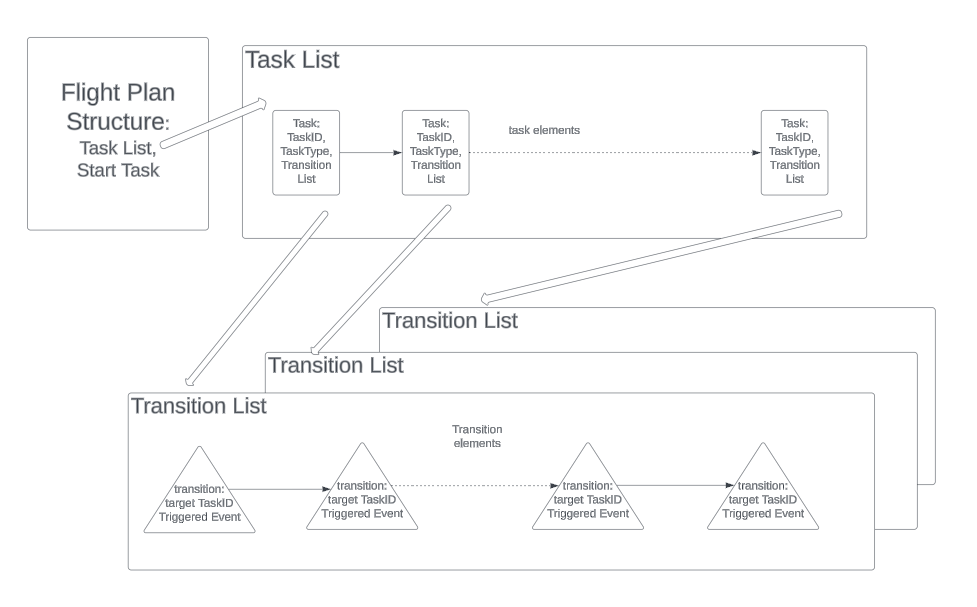
\includegraphics[width=0.8\textwidth]{Pictures/cli_auto.PNG}
    \caption{Flight Plan Structure (FPS).}
    \label{fig:cli_auto}
\end{figure}

\begin{itemize}
    \item \textbf{Flight Plan Structure (FPS)}: Comprises the start task ID and a comprehensive list of tasks. This structure serves as the backbone for task management and transition flow within the mission.
    \item \textbf{Task List}: This component includes each task object created and defined by the user, forming the operational sequence for the mission.
    \item \textbf{Task}: Every task object within the list includes a unique task ID, task type (such as detect, track, or avoid), and a list of transitions that define the flow to subsequent tasks based on specific events.
    \item \textbf{Transition List}: Contains all transitions associated with a task object, detailing the conditions under which a transition to another task is triggered.
    \item \textbf{Transition}: Each transition specifies the event that triggers it and the ID of the next task to be executed.
\end{itemize}


\section{Runtime}
\subsection{Overview}
DroneDSL requires an entry-point file created using the drone SDK to establish drone connectivity and initiate external communications. This activates the mission controller, a DroneDSL library module that oversees the entire mission. It manages the task runner, an asynchronous worker responsible for starting and stopping tasks. Tasks are performed asynchronously, executing drone commands and monitoring events through transition threads. Triggered events are reported to the mission controller, which assesses them and instructs the task runner to either switch, continue, or terminate tasks. Upon command, the task runner stops all current tasks and transitions.

\begin{figure}[H] % The 'h' here is a placement specifier (here)
    \centering % This centers the figure
    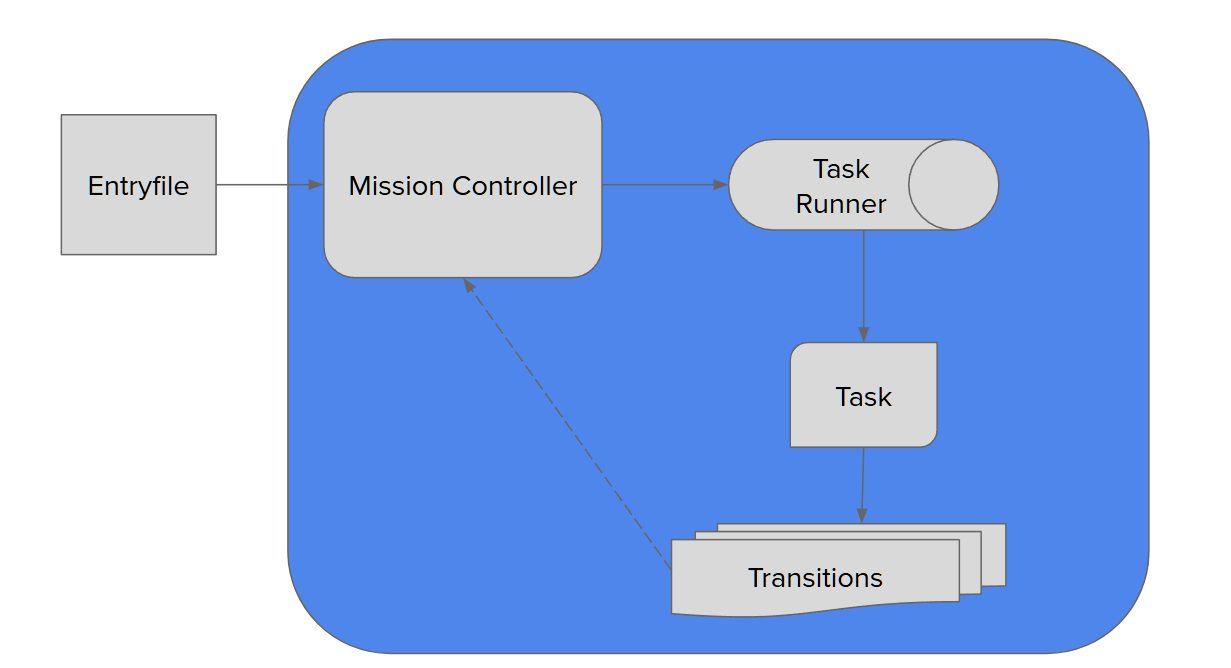
\includegraphics[width=0.8\textwidth]{Pictures/run_flow.PNG}
    \caption{Workflow Diagram for the Runtime Module.}
    \label{fig:runtime_diagram}
\end{figure}

\subsection{Components}
\begin{itemize}
    \item \textbf{Mission Controller}: Oversees the entire flight operation.
    \begin{itemize}
        \item Initiates the mission by launching the task runner and instructing the drone to take off.
        \item Modifies tasks in response to events detected during task transitions, guided by the mission creator.
        \item Concludes the mission by shutting down the task runner and directing the drone to return.
    \end{itemize}
    \item \textbf{Task Runner}: Operated by the mission controller to execute or end tasks.
    \begin{itemize}
        \item Manages a queue of tasks, executing new tasks as they are introduced.
        \item Capable of ending the current task and initiating subsequent ones.
    \end{itemize}
    \item \textbf{Mission Creator}: An automatically generated file that details the specific mission set-up by DroneDSL.
    \begin{itemize}
        \item Defines the task automata, providing a reference for the mission controller.
    \end{itemize}
\end{itemize}

} %//Some other possible sections
\chapter{Future Work}
\label{sec:future}


\section{Short Term Goals}
In the short term, the objective is to \textbf{enrich the language} of DroneDSL by introducing new tasks to broaden the variety of tasks, defining trigger events with a class-based structure similar to tasks, enabling composable conditional statements using logical operators such as "and", and incorporating the ability to add comments within the code.

Further enhancements will focus on \textbf{style and checking} features. This includes adopting a keyword style similar to SQL to improve readability and familiarity. Improvements will also be made in compilation checks by enforcing strict type validation for syntax checking, ensuring contextual accuracy through semantic checks, verifying drone compatibility to ensure equivalence with various drone models, confirming model adherence through model compatibility checks, and employing ``include" and ``extern" semantics for state verification.

Additionally, the \textbf{runtime library} will be refined by modularizing the mission architecture. This involves separating the mission creator, controller, and task runner into distinct threads from the drone SDK script, thus optimizing performance and reliability.

\section{Long Term Goals}
The current implementation of DroneDSL allows for specifying tasks based on object classes, such as detecting or tracking a person or a vehicle. An intriguing direction for further development is enhancing how classes are described to capture more complex scenarios. For instance, we might want a drone to identify a specific scene where two individuals, distinguished by attributes like clothing color, gender, and height, are shaking hands. To facilitate this, DroneDSL would need to evolve to include a system that can articulate and manage the relationships between various features within a scene, thereby allowing for a more nuanced and expressive description of detection tasks.

Currently, DroneDSL enables the execution of one task at a time. However, as some drones are capable of multitasking—e.g.performing maneuvers while simultaneously avoiding obstacles—there is a significant opportunity to expand the language's semantics to support the execution of foreground and background tasks simultaneously. This enhancement would leverage the advanced capabilities of modern drones and offer more dynamic and efficient mission planning.

While DroneDSL supports autonomous operations, manual mode remains crucial for drone operation. Enhancing DroneDSL to seamlessly transition between autonomous and manual modes would greatly increase its practicality. Since DroneDSL is a compiled language, enabling real-time interpretation during manual mode might require integrating features that allow pilots to use the language interactively. This capability would make the language more flexible and adaptable to real-time operational needs.

Another area of interest is runtime variable binding. In many drone operations, the targets of interest might not be defined during the initial compilation or mission planning stages. For example, if a pilot spots something of interest mid-mission, they should have the capability to dynamically bind this new target with the existing features detected by the drone's sensors. Developing features in DroneDSL to support such dynamic binding would enhance its utility in diverse operational contexts.

Currently, DroneDSL is limited to executing one mission at a time. To accommodate long-distance tasks, particularly for lighter drones with limited onboard power, integrating multi-hop planning capabilities is essential. This could mirror the practice of fixed-wing pilots who prepare navigation logs to plan optimized routes and manage fuel consumption. By incorporating a similar strategy into DroneDSL, the language could provide facilities for breaking down long missions into manageable segments, potentially using optimization algorithms during the compilation phase to enhance route efficiency and power management.

Lastly, considering the potential of coordinated multi-drone missions opens up another promising avenue for DroneDSL's evolution. Enabling the language to articulate and manage multiple drones working in concert could dramatically expand the scope and impact of drone technology.}
\chapter{Conclusion}
\label{sec:conclude}

This thesis introduced DroneDSL, a specialized language designed to make planning drone missions, especially for reconnaissance, more effective and easier to manage. DroneDSL simplifies how developers and pilots work with drones by creating a more user-friendly layer that handles complex tasks. It also helps developers be more efficient because they can reuse parts of their code for different projects. Unlike other drone languages that only support simple, straight-line planning, DroneDSL allows for more complex operations like loops and conditional actions. This means drones can adjust their behavior on the fly to meet changing conditions during a mission, which is a big step up from current capabilities.


In summary, DroneDSL marks an improvement in how drone missions are planned and executed. The next steps in research and development will likely expand on these foundations, exploring new ways to enhance drone capabilities for various uses .}

%==============================================================================

%-----------------------------------------------------------------------------%
% BIBLIOGRAPHY -- uncomment \nocite{*} to include items in 'mybib.bib' file
% that aren't cited in the text.  Change the style to match your
% discipline's standards.  Of course, if your bibliography file isn't called
% 'mybib.bib' you might want to change that here too :)
%-----------------------------------------------------------------------------%
%\nocite{*} - if you use this it will put EVERYTHING in your .bib file into the references even if you don't cite it in the text
%\bibliographystyle{./Bibliography/jasa} %Formats bibliography

% Set the bibliography style
\bibliographystyle{IEEEtranS} % Change to a path relative to your main .tex file or use a system-wide style

% Ensure the bibliography starts on a new page
\cleardoublepage

% Reset any changes to line spacing to default
\normalbaselines

% % Add the bibliography to the Table of Contents as a chapter
% \addcontentsline{toc}{chapter}{Bibliography}

% Specify the .bib file containing your bibliographic entries
\bibliography{./Bibliography/mybib} % Ensure the path to your .bib file is correct

%-----------------------------------------------------------------------------%
% APPENDICES -- OPTIONAL. These are just chapters enumerated by Appendix 1,
%                Appendix 2, Appendix 3...
%-----------------------------------------------------------------------------%
\appendix
\chapter{Example Mission Scripts}

This chapter provides three progressively complex examples of mission scripts using DroneDSL. These scripts illustrate the computational capabilities of DroneDSL in the context of mission planning.

\section{Appendix 1}
This basic mission script tasks a drone with patrolling a specified area once, using the "coco" deep neural network model to detect objects during the patrol. It specifies waypoints, camera settings, and operational parameters to optimize the detection process.
\begin{lstlisting}[style=customgo]
Task {
    Detect task1 {
        way_points: [(-79.9502696,40.4156737,5.0),
                     (-79.9502655,40.4154588,5.0),
                     (-79.9499142,40.4154567,5.0),
                     (-79.9499128,40.4156753,5.0),
                     (-79.9502696,40.4156737,5.0)],
        gimbal_pitch: -20.0,
        drone_rotation: 0.0,
        sample_rate: 2,
        hover_delay: 0,
        model: coco,
    }
}

Mission {
    Start task1
}
\end{lstlisting}

\section{Appendix 2}
This script depicts a more complex surveillance mission, instructing the drone to alternate between patrolling a triangular and a rectangular area using the 'coco' model. If a car is detected, the drone begins a 20-second tracking task. The mission cycle repeats with transitions based on detection and tracking outcomes. The mission ends if a tracking task loses sight of its target for 10 seconds or a detection task completes without finding its target. The path followed is illustrated in \ref{fig:appendix_1}.
\begin{lstlisting}[style=customgo]
Task {
    Detect tri {
        way_points: <Triangle>,
        gimbal_pitch: -20.0,
        drone_rotation: 0.0,
        sample_rate: 2,
        hover_delay: 0,
        model: coco,
    }
    
    Detect rec {
        way_points: <Rectangle>,
        gimbal_pitch: -20.0,
        drone_rotation: 0.0,
        sample_rate: 2,
        hover_delay: 0,
        model: coco,
    }

    Track tri_track {
        gimbal_pitch: -30.0,
        model: coco,
        class: car,
    }
    
    Track rec_track {
        gimbal_pitch: -30.0,
        model: coco,
        class: car,
    }
}

Mission {
    Start tri
    Transition (object_detection(car)) tri -> tri_track
    Transition (timeout(20)) tri_track -> rec
    Transition (object_detection(car)) rec -> rec_track
    Transition (timeout(20)) rec_track -> tri
}
\end{lstlisting}

\begin{figure}[H]
    \centering
    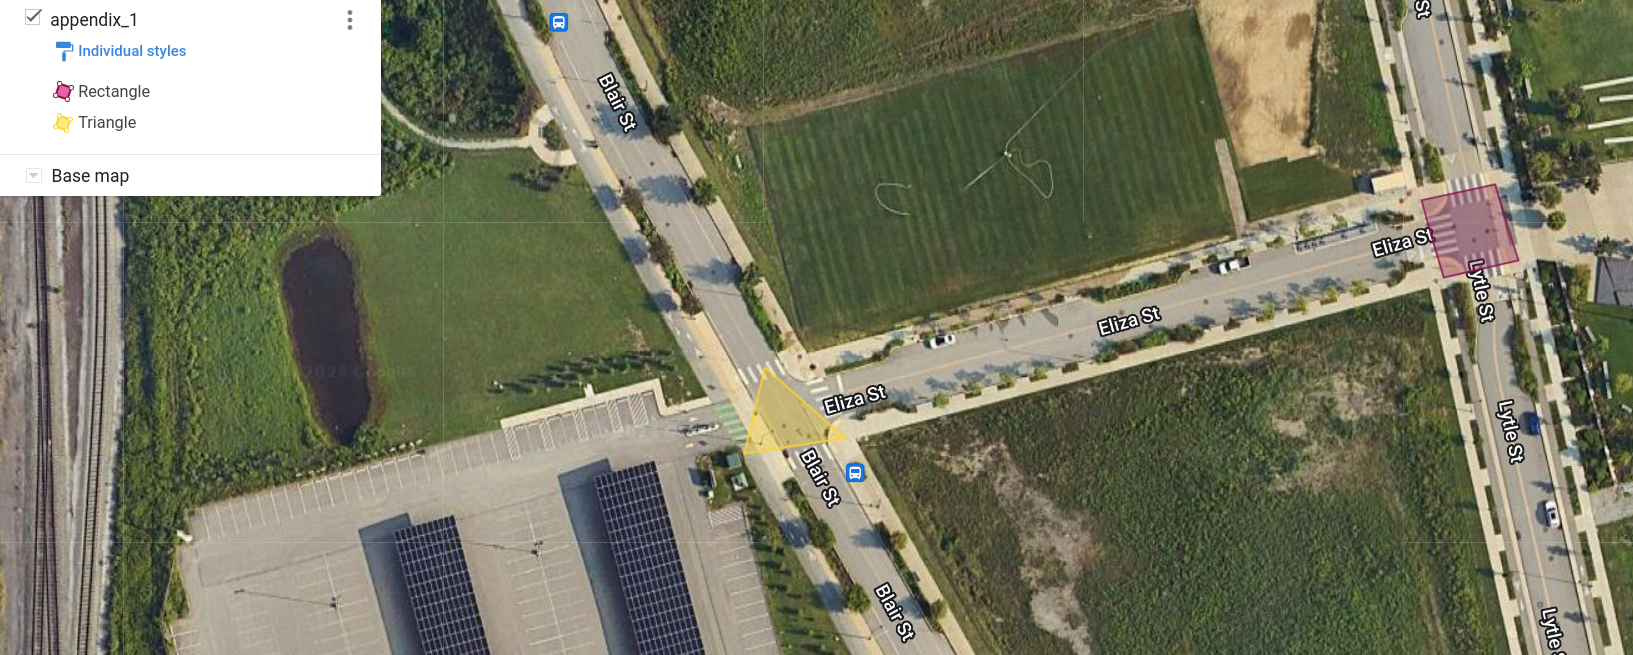
\includegraphics[width=0.8\textwidth]{Pictures/thesis_appendix_2.png}
    \caption{Illustrative Flight Route for Appendix 2.}
    \label{fig:appendix_1}
\end{figure}

\section{Appendix 3}
This mission script involves a drone navigating the Hot Metal Bridge while avoiding obstacles and subsequently monitoring pedestrian movement along the Three River Heritage Trail. Detection and tracking tasks use the 'midas' and 'visdrone' models respectively. The mission concludes when a pedestrian is out of sight for 10 seconds after being tracked. The trajectory of the mission is displayed in \ref{fig:appendix_2}.
\begin{lstlisting}[style=customgo]
Task {
    avoid task1 {
        way_points: <HotMetalBridge>
        speed: 1.0
        model: midas
        altitude: 8.0
    }

    Detect task2 {
        way_points: <ThreeRiverHerritageTrail>
        gimbal_pitch: -20.0,
        drone_rotation: 0.0,
        sample_rate: 2,
        hover_delay: 0,
        model: visdrone,
    }

    Track task3 {
        gimbal_pitch: -30.0,
        model: visdrone,
        class: pedestrian,
    }
}

Mission {
    Start task1
    Transition (object_detection(pedestrian)) task2 -> task3
    Transition (done) task2 -> task2
    Transition (done) task1 -> task2
}
\end{lstlisting}

\begin{figure}[H]
    \centering
    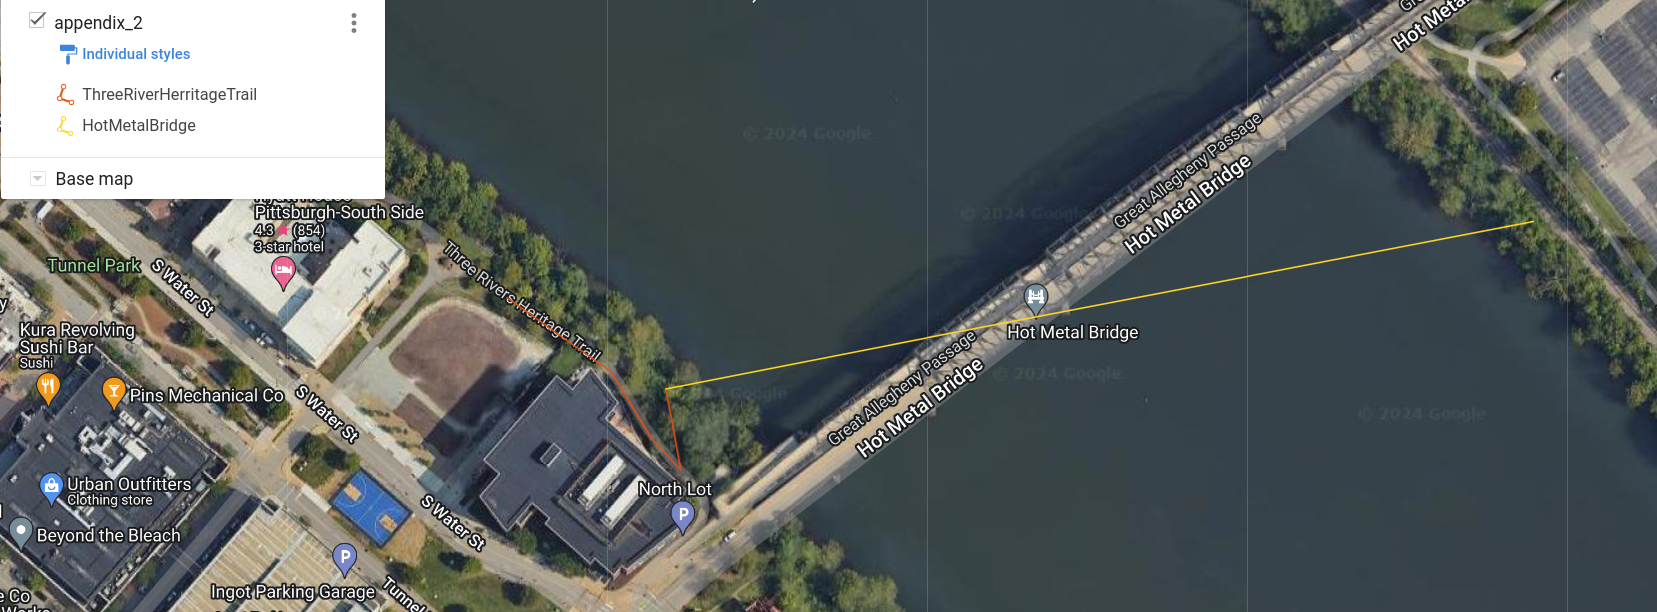
\includegraphics[width=0.8\textwidth]{Pictures/thesis_appendix_3.png}
    \caption{Flight Route for Appendix 3.}
    \label{fig:appendix_2}
\end{figure}}
% Start with '\chapter{Title}'
%You can always add more appendices here if you want
% You're done :)
\end{document}
